\documentclass[]{article}
\usepackage{ctex}
\usepackage{graphicx}
\usepackage{listings}
\usepackage{fontspec}
\newfontfamily\cn{Courier New}
\lstset{
	xleftmargin=2em,
	%numbers=left,
	framexleftmargin=10mm,
    frame=none,
    language=C++,
	basicstyle=\cn,
	%keywordstyle=\bf\cn,
	identifierstyle=\cn,
	numberstyle=\cn,
	commentstyle=\cn,
	stringstyle=\cn,
	showstringspaces=false,
	breaklines=true, 
	breakautoindent=true,
	breakindent=2em, 
	tabsize=4,
}

%opening
\title{DNS中继服务器的实现}
\author{房庆凯}

\begin{document}

\maketitle

\section{题目概述}
设计一个DNS服务器程序,读入「域名-IP地址」对照表,当客户端查询域名对应的IP地址时,用域名检索该对照表,三种检索结果:
\begin{itemize}
    \item 检索结果为IP地址0.0.0.0,则向客户端返回「域名不存在」的报错消息(不良网站拦截功能)
    \item 检索结果为普通IP地址,则向客户返回这个地址(服务器功能)
    \item 表中未检到该域名,则向因特网DNS服务器发出查询,并将结果返给客户端(中继功能)
\end{itemize}

\section{理论基础}
    \subsection{DNS简介}
        由于IP地址太过繁琐,使用IP地址来识别参与分布式应用的主机十分困难,因此互联网支持使用主机名称来识别主机。
        为了使用如TCP和IP等协议,主机名称通过称为名称解析的过程转换成IP地址,互联网中最普遍、最重要的一种名称解析是采用分布式数据库系统,即人们熟知的域名系统 (DNS)。
        DNS作为互联网上的应用程序运行,它使用IPv4或IPv6(或者两者都使用)。

        DNS是一个分布式的客户机/服务器网络数据库,TCP/IP应用程序使用它来完成主机名称和IP地址之间的映射(反之亦然),从而提供各种服务。
        DNS提供了允许客户机和服务器相互通信的协议,并且也提供了服务器之间交互信息的协议。

        在请求TCP打开一个连接或使用UDP发送一个单播数据报之前,应用程序必须将主机名称转换为IPv4与/或IPv6地址。TCP和IP协议实现对DNS一无所知,它们只对地址进行操作。


    \subsection{DNS名称空间与命名语法}
        DNS中使用的所有的名称集合构成了DNS名称空间。
        当前的DNS名称空间是一棵域名树,位于顶部的树根未命名。树的最高层是所谓的顶级域名(TLD)。

        DNS名称树中TLD下面的名称进一步划分成组,称为子域名,例如中国的大部分教育站点使用后缀 .edu.cn。
        一个域名包含一系列的由点分开的标签。名称代表名称层级中的一个位置,句点是层次结构分隔符,并且按名称中自右至左的顺序沿树下降。每个标签最多可到63个字符长。
        
    \subsection{DNS服务器和区域}
        部分DNS名称空间的管理责任分配给个人或组织,他们通过安置DNS服务器来存储名称空间的相关信息,以便互联网用户查询名称。
        服务器的集合形成了DNS本身,它是一个提供名称到地址的映射的分布式系统。

        在DNS服务器的语言中,管理授权的单位称为区域。一个区域是DNS名称空间的一棵子树,它可以独立管理而不受其他区域影响。
        每一个域名都存在于某个区域中,即使是TLD,它也存在于根区域中。
        每当一个新记录添加到区域中时,该区域的DNS管理员为该新条目分配一个名称和附加信息(通常是IP地址),并且将这些信息保存到名称服务器的数据库中。

    \subsection{缓存}
        大部分的DNS服务器会缓存它们学习的区域信息,直到生存时间(TTL)的时间限制为止。使用缓存的信息来应答查询请求,可以大大减少DNS消息的流量。
        
        每个DNS记录有自己的TTL以控制其缓存的时间,这些值在必要时由区域管理员设置和更改。TTL指明了DNS中一个映射在任何地方能够被缓存的时间,如果一个区域变化了,在TTL失效之前网络中仍存在缓存的数据,这可能导致不正确的DNS解析过程。
        因此一些想要改变区域内容的管理员,会在更改之前首先减少TTL的值。

        缓存同时适用于成功的解析和不成功的解析(否定缓存),如果一个请求返回域名不存在时,将该事实缓存下来,之后再次请求该不存在的域名时可以直接返回,从而降低互联网流量。
    
    \subsection{DNS协议}
        DNS协议主要由两个主要部分组成,对DNS特定名称查询的查询/响应协议和DNS服务器用于交换数据库记录的协议(区域传输)。最典型的用法是使用一个简单的查询/响应来查找域名对应的IPv4/IPv6地址。

        \subsubsection{DNS消息格式}
            基本的DNS消息格式如下所示。
            \begin{figure}[ht]
                \centering
                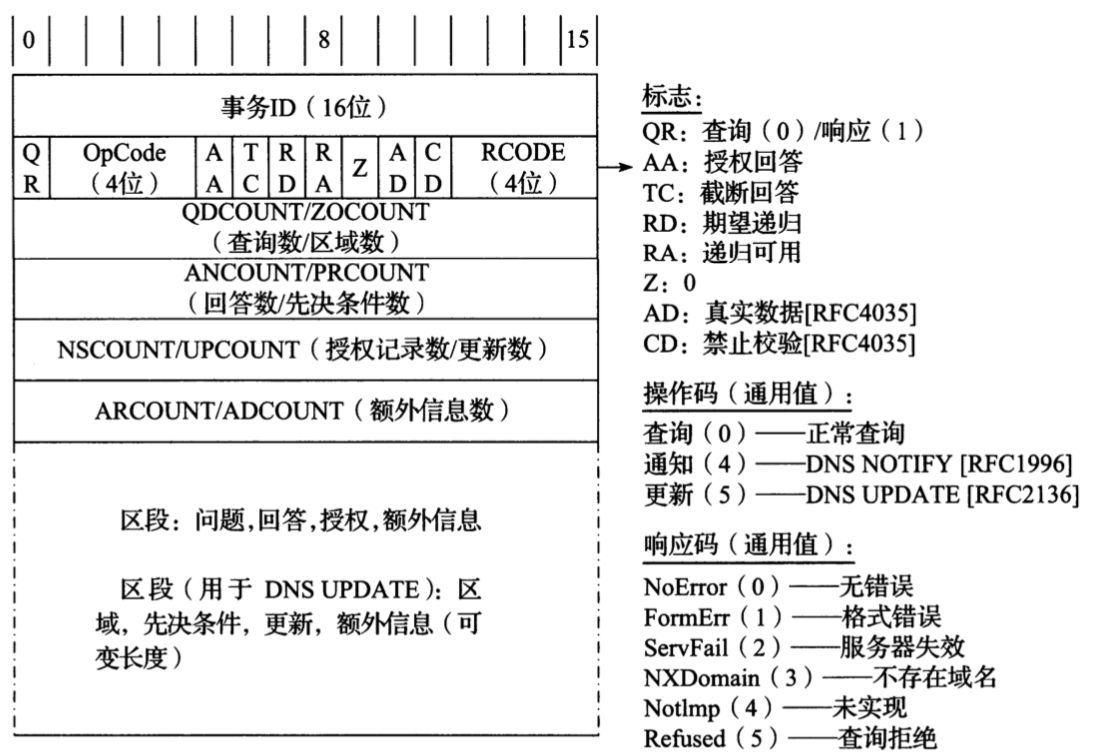
\includegraphics[scale=0.6]{dns.png}
                \caption{DNS消息格式}
            \end{figure}
            基本的DNS消息格式以固定的12字节头部开始,其后跟随4个可变长度的区段:问题、回答、授权记录、额外记录。
            除了第一个区段,其他都包含一个或多个资源记录。

            在固定长度的头部中,事务ID字段由客户端设置,由服务器返回。客户端使用它来匹配响应和查询。
            
            第二个16位的字包含一些标志和其他的子域。
            从最左边的位开始,QR是1位的字段:0表示查询消息;1表示响应消息。
            下一个是操作码(OpCode),4位的字段。查询和响应中的正常值是0(标准查询)。其他值为:4(通知),5 (更新)。其他值(1 - 3)是弃用的,在运作过程中不会出现。
            下一个是AA位字段,表示授权回答(与缓存回答相对)。
            TC是1位的字段,表示「可截断的」。使用UDP时,它表示当应答的总长度超过512字节时,只返回前512个字节。
            RD是1位字段,表示「期望递归」,该字段可以在一个查询中设置,并在响应中返回。
            它告诉服务器执行递归查询。如果该字段没有设置,且被请求的名称服务器没有授权回答,则被请求的名称服务器就返回一个可以联系获取回答的其他名称服务器的列表。此时,全部的查询可能通过联系其他名称服务器来继续。这被称为迭代查询。
            RA是1位字段,表示「递归可用」。如果服务器支持递归查询,则在响应中设置该字段。根服务器一般不支持递归,因此强制客户端执行迭代查询来完成名称解析。
            目前Z位字段必须是0,但是为将来使用而保留。
            如果包含的信息是已授权的,则AD位字段设置为真,如果禁用安全检查,则CD位设置为真。
            响应码(RCODE)是一个4位的返回码字段。通常的值为0(没有差错)和3(名称差错或「不存在域名」,写作NXDomain)。名称错误只会由授权名称服务器返回,表示在查询中指定的域名不存在。

            随后的4个字段均为16位,说明了组成DNS消息的问题、回答、授权和额外信息区段中条目的数目。对于查询消息,问题的数目通常为1,其他三项计数则为0。对于应答消息,回答的数目至少为1。问题区段有名字、类型和类。所有的其他区段都包含零个或多个RR。RR包含名字、类型和类信息,也包含控制数据缓存时间的TTL值。

            \paragraph{名称和标签}
                DNS消息末尾的可变长度区段包含问题、回答、授权信息和额外信息。每一个问题和RR以它所涉及的名称开始。
                每个名称由一系列的标签组成。标签类型有两种:数据标签和压缩标签。数据标签包含构成一个标签的字符;压缩标签充当指向其他标签的指针。当相同字符串的多个副本在多个标签中出现时,压缩标签有助于节省DNS信息的空间。

            \paragraph{数据标签}
                每个数据标签以1字节的计数开始,该计数指定了紧随其后的字节数目,名称以值为0的字节结束。例如,名称 www.pearson.com 的编码如下所示。
                \begin{figure}[ht]
                    \centering
                    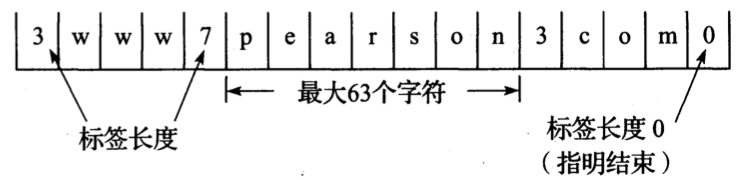
\includegraphics[scale=0.6]{datalabel.png}
                    \caption{数据标签}
                \end{figure}
                对于数据标签来说,每个标签的长度字节的值必须在0到63之间。

            \paragraph{压缩标签}
                在许多情况下,DNS响应消息在回答、授权以及与相同域名相关的额外信息区段中携带信息。
                如果使用了数据标签,当涉及相同的名称时,DNS消息中的相同字符就会重复。
                为了避免这种冗余和节省空间,使用了一种压缩机制。DNS消息中,在域名的标签部分能出现的任意位置,前面的单一计数字节(通常在0和63之间)的2个高位置1,剩余的位与随后的字节中的位组合形成一个14位的指针(偏移量)。偏移量给出了距离DNS消息开始处的字节数,在那里可以找到一个用于替代压缩标签的数据标签(称为压缩目标)。因此压缩标签能够指向距离开始处多达16383个字节的位置。
                例如,域名 usc.edu 和 ucla.edu 的压缩编码如下所示。
                \begin{figure}[ht]
                    \centering
                    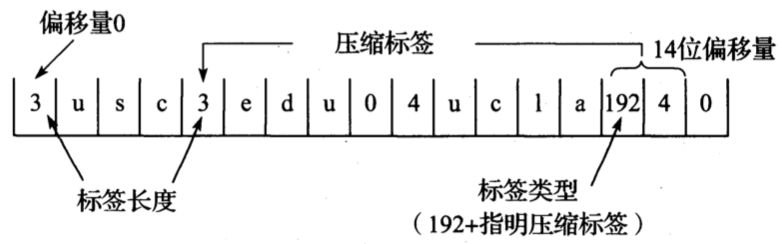
\includegraphics[scale=0.6]{ziplabel.png}
                    \caption{压缩标签}
                \end{figure}
        
        \subsubsection{UDP}
            对于UDP来说,DNS的知名端口号是53,常见的格式是使用如下所示的UDP/IPv4的数据报结构。
            \begin{figure}[ht]
                \centering
                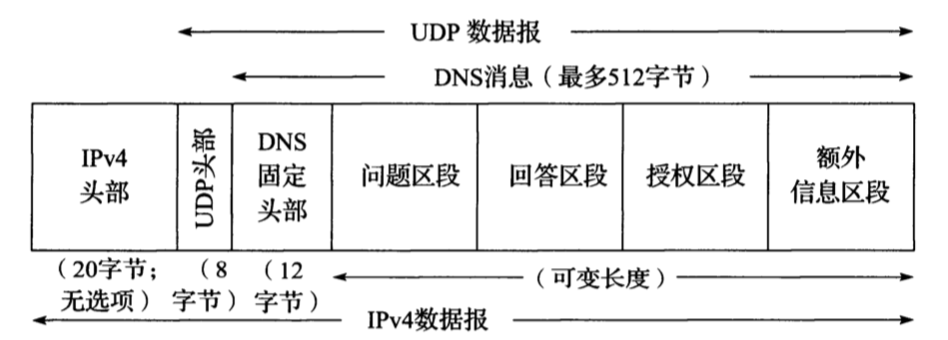
\includegraphics[scale=0.6]{udp.png}
                \caption{UDP/IPv4数据报}
            \end{figure}

        \subsubsection{查询字段格式}
            查询字段中每个问题的格式如下所示。
            \begin{figure}[ht]
                \centering
                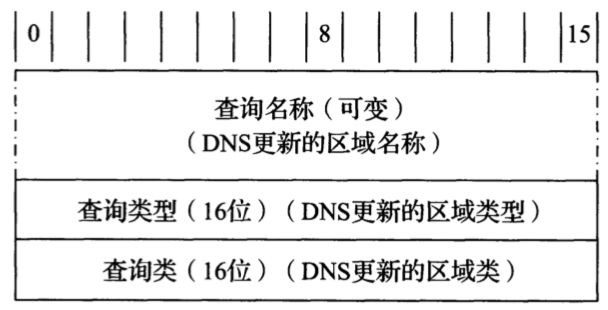
\includegraphics[scale=0.6]{question.png}
                \caption{DNS消息中的查询字段}
            \end{figure}
            查询名称是要被查询的域名,使用我们之前描述的标签的编码。
            每个问题都有查询类型和查询类。类的值是1、 254或255,分别表示互联网类、没有类或所有类,其他值通常不用于TCP/IP网络。
            查询类型字段包含一个值,指明正在执行的查询类型。最常见的查询类型是A(如果启用IPv6的DNS解析,则是AAAA),这意味着需要一个与查询名称对应的IP地址。

        \subsubsection{回答、授权和额外信息字段格式}
            DNS信息中的最后三个区段——回答、授权和额外信息,包含RR的集合。每个资源记录的格式如下所示。
            \begin{figure}[ht]
                \centering
                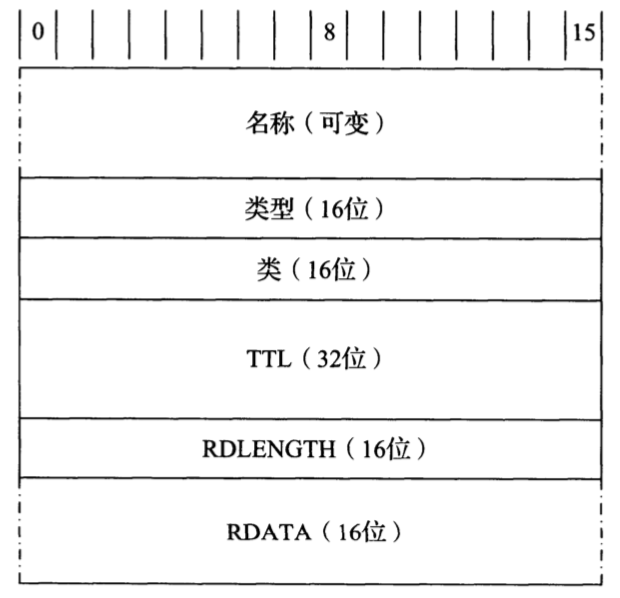
\includegraphics[scale=0.6]{rr.png}
                \caption{DNS资源记录格式}
            \end{figure}
            名称字段是随后的资源数据对应的域名,它与我们之前描述的名称和标签的格式相同。
            类型字段指定为RR类型代码中的一个。这些和我们之前描述的查询类型值相同。对于互联网数据来说,类字段是1。 
            TTL字段是RR可以被缓存的秒数。资源数据长度字段指定了资源数据字段中包含的字节数。数据的格式取决于类型。例如,A记录(类型1)在RDATA域中有一个32位的IPv4地址。

\section{功能设计}
    \subsection{不良网站拦截}
        当在本地域名-IP记录表中查找到的IP为0.0.0.0时,即将报文的响应码设置为3,然后发送至客户端,表示当前查找的域名不存在。
        因此,我们只要在本地域名-IP记录表中,将不良网站的IP地址设置为0.0.0.0,就可以实现不良网站的拦截功能了。
    \subsection{服务器}
        当在本地域名-IP记录表中匹配到所查询的域名,且检索结果为普通IP地址时,表示我们在本地表中找到了域名对应的地址,将该地址置入报文的ANSWER字段并将报文返回给客户端即可。
    \subsection{中继}
        当在本地域名-IP记录表中匹配不到所查询的域名时,即将该报文转发到远端服务器。

        为了实现多客户端并发查询,即允许第一个查询尚未得到答案前就启动处理另外一个客户端的查询请求。
        我们需要在中继服务器中进行ID的转换,并用一个查询记录表将新ID$\ \to$旧ID的映射关系记录下来。当收到一个来自远端服务器的报文时,根据查询记录表确定旧ID以及客户端的地址,将ID字段修改为之前的ID,发送回客户端即可。
    \subsection{缓存}
        为减少DNS消息的流量,我为DNS增加了缓存的功能。缓存的信息保存在 cache.txt 中,每一个条目是形如<IP、域名、截止时间>的三元组。
        当我们的DNS中继服务器收到远端服务器的DNS消息时,则从DNS消息的回答字段中提取出IP、域名、TTL,并根据TTL和当前的时间计算出截止时间,然后将该三元组插入缓存表中。

        之后再收到客户端的查询时,我们检查本地的域名-IP记录表和缓存表,如果成功找到则将IP返回,否则再向远端服务器发送询问。注意每次在缓存表中查询时要将其中已经超时的表项删除,保证查到的表项都是有效记录。

\section{模块划分}
    \subsection{socketManager模块}
        该模块主要负责网络通信。首先建立一个socket并绑定到UDP的53号端口,接收来自53号端口的所有报文。
        
        该模块定义的函数如下:
        
        \begin{lstlisting}
int socketManager::recvBuffer(uint8_t *buffer, sockaddr_in &senderAddr, time_t &recvTime)
void socketManager::sendBuffer(uint8_t *buffer, int bufferSize, sockaddr_in recvAddr)
        \end{lstlisting}

        \verb@recvBuffer()@的作用是,接收一个报文,将其内容存储到buffer中,并将发送方的地址和到达时间分别存储到senderAddr和recvTime中。
        
        \verb@sendBuffer()@的作用是,发送一个报文,其中报文的内容现在存储在buffer中,bufferSize为buffer的大小,recvAddr为接收方的地址。
        
    \subsection{nameTable模块}
        该模块主要负责本地域名-IP对照表以及缓存表的相关操作,使用的数据结构如下:
        \begin{lstlisting}
struct nameItem {
    std::string name;
    uint32_t IP;
    time_t ddl;
};

struct ddlcmp {
    bool operator()(nameTable::nameItem lhs, nameTable::nameItem rhs) {
        return lhs.ddl < rhs.ddl;
    }
};

std::multiset<nameTable::nameItem, nameTable::ddlcmp> ddlSet;
std::map<std::string, nameTable::nameItem> domainMap;
        \end{lstlisting}

        结构体 nameItem 存储了一个三元组<IP、域名、截止时间>,domainMap 使用了map来进行从域名到表项的映射;
        ddlSet 使用了 multiset 来维护当前的所有表项,并按照截止时间(ddl)排序,便于我们剔除超时的表项。

        该模块定义的函数如下:

        \begin{lstlisting}
void read_hostfile();
void read_cachefile();
void write_file();
void clearTimeoutItem();
void insertItem(std::string name, uint32_t IP, time_t ddl);
bool query(std::string name, uint32_t &IP, time_t &ddl);            
        \end{lstlisting}

        其中,\verb@read_hostfile()@和\verb@ read_cachefile()@用于从本地的dnsrelay.txt以及cache.txt中读取数据来构建表项,并加入到 ddlSet 和 domainMap 中。
        需要注意的是,对于从 dnsrelay.txt 中读取的表项,我们将其 ddl 设为 LONG\_MAX,即表示其永远不会超时。
        
        \verb@write_file()@ 用于向 cache.txt 中写入新表项,以更新缓存表的内容。

        \verb@query()@ 使用 domainMap 来查找域名 name 对应的表项,若在本地域名-IP对照表或缓存表中找到对应表项,则将对应的IP地址和截止时间存储到IP和ddl中,并返回true;否则返回false。

        \verb@insertItem()@ 用于加入一个表项。

        \verb@clearTimeoutItem()@ 将当前缓存表中的所有超时表项删除。

    \subsection{recordTable模块}
        该模块主要负责DNS中继服务器中查询记录表的相关操作,使用的数据结构如下:
        \begin{lstlisting}
const std::chrono::seconds timeout = std::chrono::seconds(10);            

struct record {
    uint16_t id;
    sockaddr_in senderAddr;
    std::chrono::system_clock::time_point arriveTime;
};

uint16_t currentID;
std::vector<std::pair<uint16_t, recordTable::record> > table;
        \end{lstlisting}
        
        DNS服务器进行中继时,需要进行ID的转换,为了保证远端服务器返回的报文能够发回正确的客户端,我们需要记录下其旧ID以及客户端地址。

        结构体record存储了一个三元组<旧ID,客户端地址,到达时间>,currentID 表示新ID,每次插入一条新记录都递增,保证发往远端服务器的ID独一无二。
        
        table 即我们的查询记录表,使用vector存储二元组<新ID,record>。对于当前所有已发往服务器但仍未收到应答的查询,在该表中都存在一个表项。

        该模块定义的函数如下:

        \begin{lstlisting}
uint16_t insertRecord(message msg);
bool findRecord(uint16_t id, record &tmpRecord);
void deleteTimeoutRecord();
        \end{lstlisting}

        \verb@insertRecord()@ 用于向 table 中加入一条记录,相关信息存储在报文 msg 中。

        \verb@findRecord()@ 用于当收到一条远端服务器返回的应答时,在table中查询其对应的旧ID和客户端地址。

        \verb@deleteTimeoutRecord()@ 用于删除超时表项。由于 UDP 不可靠,当table中的某一个表项对应的询问超过一定时间仍未收到应答时,我们认为此时发生了丢包,将该表项从 table 中删除。

    \subsection{message 模块}
        该模块主要负责结构体和字节流的转换,由于我们通过UDP发送和接收的都是字节流,而处理报文(如添加、修改某个字段等)时我们使用的是结构体,因此二者之间的转换必不可少。该模块使用的数据结构如下:

        \begin{lstlisting}
struct HEADER {
    uint16_t ID;

    bool QR;
    uint8_t OPCODE;
    bool AA;
    bool TC;
    bool RD;
    bool RA;
    uint8_t ZERO;
    uint8_t RCODE;

    uint16_t QDCOUNT;
    uint16_t RRCOUNT[3];
};

struct QUESTION {
    std::string QNAME;
    uint16_t QTYPE;
    uint16_t QCLASS;
};        

struct RESOURCE_RECORD {
    std::string NAME;
    uint16_t TYPE;
    uint16_t CLASS;
    uint32_t TTL;
    uint16_t RDLENGTH;
    std::vector<uint8_t> RDATA;
};

enum RRTYPE {
    ANSWER, AUTHORITY, ADDTIONAL
};

std::vector<QUESTION> question;
std::vector<RESOURCE_RECORD> RR[3];
HEADER header;
uint8_t *startPos;
sockaddr_in senderAddr;
        \end{lstlisting}

        HEADER、QUESTION、RESOURCE\_RECORD 即对照DNS消息格式、问题字段格式、RR字段格式来定义的结构体。对于不定长的 RDATA、question、RR 字段我们均使用 vector 来存储。

        startPos 表示该条 DNS 消息在缓冲区中的起始地址,用于压缩标签的解析。

        senderAddr 表示该条消息的发送方,用于发送回复时确定接收方地址。

        该模块定义的函数如下:
        \begin{lstlisting}
static std::string transName(std::string name);

void unpackName(uint8_t *&ptr, std::string &name);

void buffer2Struct(uint8_t *ptr);
void buffer2Header(uint8_t *&ptr);
void buffer2Question(uint8_t *&ptr);
void buffer2RR(uint8_t *&ptr, message::RRTYPE type);

void struct2Buffer(uint8_t *ptr, int &bufferSize);
void header2Buffer(uint8_t *&ptr, int &bufferSize);
void question2Buffer(uint8_t *&ptr, int &bufferSize);
void RR2Buffer(uint8_t *&ptr, int &bufferSize, RRTYPE type);

void getUint16(uint16_t &var, uint8_t *&ptr);
void getInt32(uint32_t &var, uint8_t *&ptr);

void putUint16(uint16_t var, uint8_t *&ptr, int &bufferSize);
void putInt32(uint32_t var, uint8_t *&ptr, int &bufferSize);};
        \end{lstlisting}

        \verb@buffer2Struct()@ 表示将当前 buffer 中的字节流提取到结构体 msg 中,
        这是分别通过调用函数 \verb@buffer2Header()@、\verb@buffer2Question()@、\verb@buffer2RR()@ 来实现的。将结构体转换成字节流的函数与之类似。

        \verb@getUint16()@ 表示从当前指针处读一个 16 位的无符号数,并存储到 var 中。\verb@getInt32()@ 同理。
        
        \verb@putUint16()@ 表示将var中的 16 位无符号数存储到当前指针处。\verb@putInt32()@ 同理。
        
        \verb@unpackName()@ 用于解析压缩标签,将其转换成普通的标签。

        \verb@transName()@ 用于将标签转换成点分形式的域名。

    \subsection{Parser模块}
        Parser模块负责主要的业务逻辑,大体思想是通过socket不断接收来自53号端口的报文,然后对该报文进行解析,并发送相应的应答包。

        我们需要存储一些必要的信息,如下所示:

        \begin{lstlisting}
uint8_t *buffer;
int bufferSize;
time_t recvTime;
message msg;
sockaddr_in serverAddr;
        \end{lstlisting}

        buffer 存储当前报文的字节流,buffersize 表示 buffer 的大到小,recvTime 表示收到当前报文的时间。
        msg 表示当前报文的结构体,serverAddr 表示当前报文的发送方地址。

        该模块定义的函数如下:
        
        \begin{lstlisting}
void receive();
void parseRequest();
void parseResponse();
void sendToServer();
void addAnswerSection(uint32_t IP, std::string name, time_t ddl);
        \end{lstlisting}

        \verb@receive()@ 通过调用 socketManager 模块的 \verb@recvBuffer()@ 来接收一个报文,并根据该报文的类型来判断接下来如何处理,具体如下:
        
        \begin{itemize}
            \item REQUEST:若报文的 QR 和 OPCODE 字段均为 0,表示这是一条询问。对于这种报文,我们进入 \verb@parseRequest()@ 部分。
            \item RESPONSE:若报文的 QR 字段为 1,表示这是一条应答。对于这种报文,我们进入 \verb@parseResponse()@ 部分。
            \item OTHER:如果不是前两种报文,我们的 DNS 中继服务器是无法进行处理的,直接发往远端服务器。
        \end{itemize}

        \verb@parseRequest()@ 为请求处理逻辑,若我们在本地的域名-IP对照表或cache表中查询成功,则通过\verb@addAnswerSection()@添加应答字段,并将报文返回客户端即可。
        若查询失败,则发往远端服务器进行查询。

        \verb@parseResponse()@ 为应答处理逻辑,当我们收到一条来自远端服务器的应答时,首先在查询记录表中找到相应的 record,找到客户端的地址,进行IP的转换,然后将报文发送回客户端即可。

        \verb@sendToServer()@ 即发往远端服务器,当我们收到的报文在本地无法成功处理时,就需要调用该函数发往远端服务器进行处理。

        \verb@addAnswerSection@ 即在当前报文中添加一个应答字段,将我们在本地查询到的 IP 和 TTL 等字段置入,并设置相关标志位。

\section{软件流程图}
    软件流程图如下所示。
    \begin{figure}[ht]
        \centering
        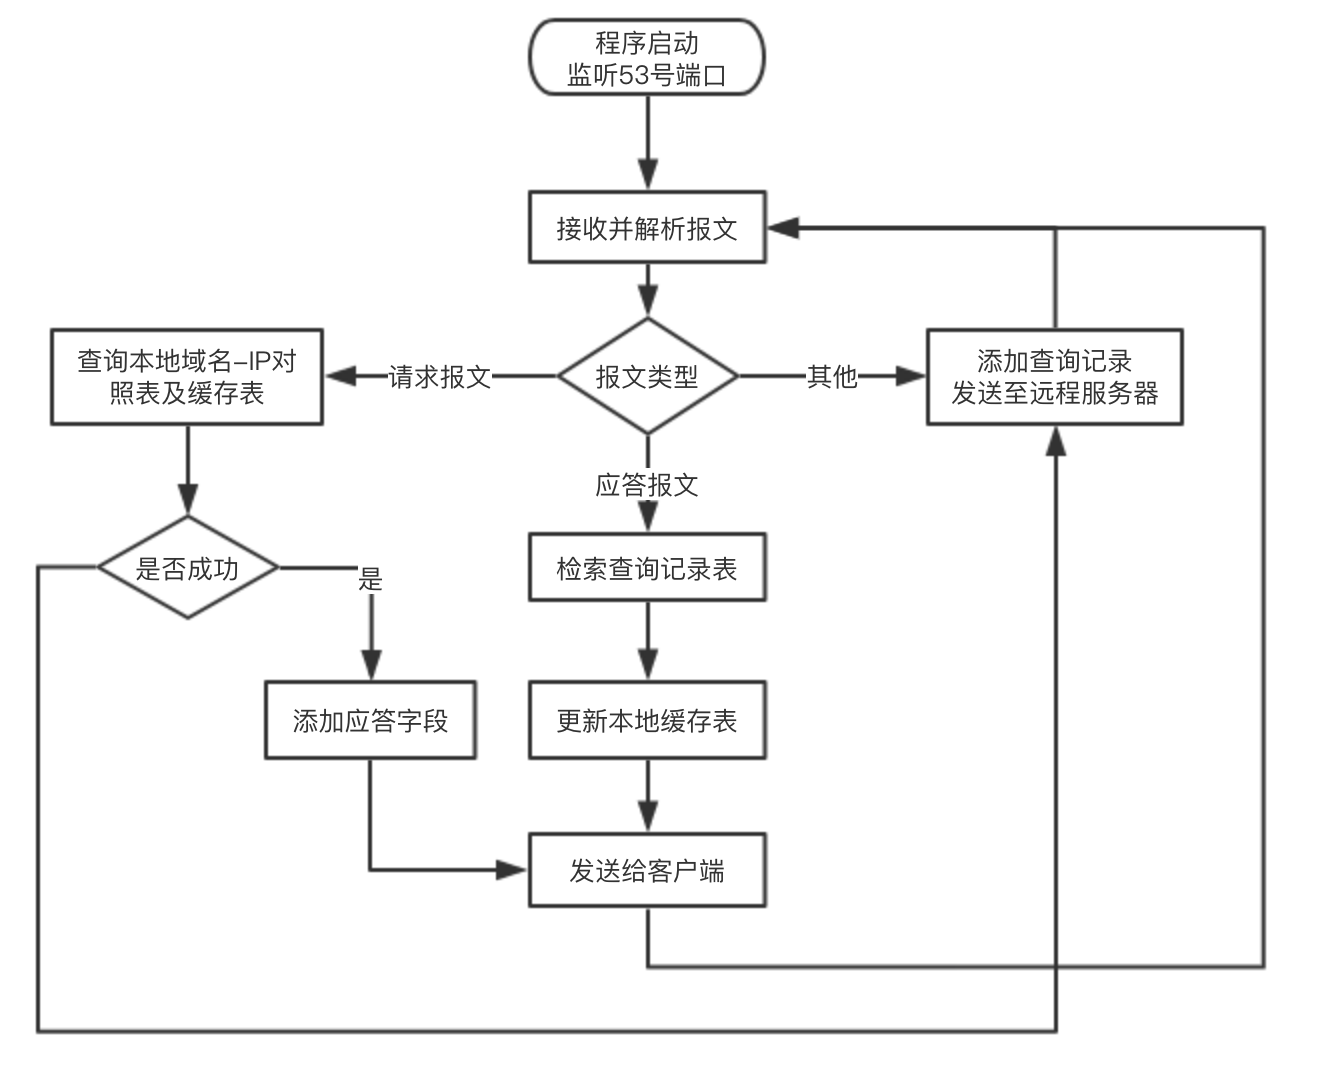
\includegraphics[scale=0.4]{flowchart.png}
        \caption{软件流程图}
    \end{figure}

\section{测试用例及运行结果}
    \subsection{使用nslookup测试}
        首先使用 nslookup 连接 DNS 服务器:
            \begin{lstlisting}
> nslookup - 127.0.0.1
            \end{lstlisting}
        \subsubsection{不良网站拦截功能}
            在 dnsrelay.txt 中,域名 cctv1.net 对应的 IP 地址为 0.0.0.0,我们输入 cctv1.net,返回 NXDOMAIN,即域名不存在,表示我们成功拦截了该网站。
            
            \begin{lstlisting}
> cctv1.net
Server:		127.0.0.1
Address:	127.0.0.1#53

** server can't find cctv1.net: NXDOMAIN
            \end{lstlisting}
        
        \subsubsection{服务器功能}
            在 dnsrelay.txt 中,存在表项 \verb@210.242.125.98 scholar.google.com@,因此我们输入 scholar.google.com,发现可以返回该 IP 地址,表示我们成功实现了服务器功能。
            
            \begin{lstlisting}
> scholar.google.com
Server:		127.0.0.1
Address:	127.0.0.1#53

Name:	scholar.google.com
Address: 210.242.125.98
            \end{lstlisting}

        \subsubsection{中继功能}
            我们访问一个 dnsrelay.txt 中没有的网站,输入 stackoverflow.com,通过请求远端服务器,我们成功获得了 IP 地址,表示我们成功实现了中继功能。

            \begin{lstlisting}
> stackoverflow.com
Server:		127.0.0.1
Address:	127.0.0.1#53

Non-authoritative answer:
Name:	stackoverflow.com
Address: 151.101.65.69
Name:	stackoverflow.com
Address: 151.101.193.69
Name:	stackoverflow.com
Address: 151.101.129.69
Name:	stackoverflow.com
Address: 151.101.1.69
            \end{lstlisting}
        
    \subsection{测试网络连通情况}
        将本机的 DNS 修改为 127.0.0.1,然后输入以下命令清空 DNS 缓存。
        \begin{lstlisting}
sudo dscacheutil -flushcache
        \end{lstlisting}

        启动程序,此时电脑仍然可以正常上网并进行域名解析,表示我们的DNS工作正常。

        现在我们使用 ping 命令来测试网络联通情况。

        \subsubsection{不良网站拦截功能}
            我们 ping 一下 cctv1.net,提示域名无法解析,表示我们实现了拦截功能。

            \begin{lstlisting}
> ping cctv1.net                
ping: cannot resolve cctv1.net: Unknown host
            \end{lstlisting}

        \subsubsection{服务器功能}
            我们 ping 一下 scholar.google.com,网络连通状况良好,表示我们成功实现了服务器功能。

            \begin{lstlisting}
> ping scholar.google.com
PING scholar.google.com (216.58.194.223): 56 data bytes
64 bytes from 216.58.194.223: icmp_seq=0 ttl=46 time=178.463 ms
64 bytes from 216.58.194.223: icmp_seq=1 ttl=46 time=176.278 ms
64 bytes from 216.58.194.223: icmp_seq=2 ttl=46 time=170.717 ms
64 bytes from 216.58.194.223: icmp_seq=3 ttl=46 time=176.301 ms
64 bytes from 216.58.194.223: icmp_seq=4 ttl=46 time=171.597 ms

--- scholar.google.com ping statistics ---
5 packets transmitted, 5 packets received, 0.0% packet loss
round-trip min/avg/max/stddev = 170.717/174.671/178.463/2.990 ms
            \end{lstlisting}

        \subsubsection{中继功能}
            我们 ping 一下 stackoverflow.com,网络连通状况良好,表示我们成功实现了中继功能。

            \begin{lstlisting}
> ping stackoverflow.com
PING stackoverflow.com (151.101.65.69): 56 data bytes
64 bytes from 151.101.65.69: icmp_seq=0 ttl=48 time=179.431 ms
64 bytes from 151.101.65.69: icmp_seq=1 ttl=48 time=180.169 ms
64 bytes from 151.101.65.69: icmp_seq=2 ttl=48 time=174.372 ms
64 bytes from 151.101.65.69: icmp_seq=3 ttl=48 time=174.445 ms
64 bytes from 151.101.65.69: icmp_seq=4 ttl=48 time=174.245 ms

--- stackoverflow.com ping statistics ---
5 packets transmitted, 5 packets received, 0.0% packet loss
round-trip min/avg/max/stddev = 174.245/176.532/180.169/2.679 ms                
            \end{lstlisting}

    \subsection{局域网上其他计算机工作}
        查看本机的IP地址为10.122.254.2,将舍友电脑的DNS地址设置为10.122.254.2,发现可以正常上网,使用 ping 测试发现网络连通状况良好。

    \subsection{缓存功能测试}
        仍然使用 nslookup 来测试,首先访问一个本地没有的域名 www.bv2008.cn,根据输出的调试信息可以发现,我们通过调用远端服务器获得了该域名的 IP 地址。

        调用完毕后,可以发现 cache.txt 中多了一条记录:
        
        \verb@103.83.46.7 www.bv2008.cn 1562786565@

        1562786565 表示的是截止时间,该时间的单位是自1970年1月1日0点到现在的秒数。只要当前时间小于截止时间,则该条缓存记录有效。

        使用 nslookup 获得的结果如下,可以看出第二次访问解析该域名时直接从本地缓存返回了IP地址。

        \begin{lstlisting}
> www.bv2008.cn
Server:		127.0.0.1
Address:	127.0.0.1#53

Non-authoritative answer:
Name:	www.bv2008.cn
Address: 103.83.46.7
> www.bv2008.cn
Server:		127.0.0.1
Address:	127.0.0.1#53

Name:	www.bv2008.cn
Address: 103.83.46.7
        \end{lstlisting}

\section{调试中遇到并解决的问题}
    \subsection{网络通信}
        要想实现DNS,网络通信是基础,由于要实现多客户端并发,开始时我的思路是使用多线程来解决问题,即为每个发往远端服务器的消息都开一个线程。
        但经过我的一番思考,多客户端并发完全可以通过单线程来解决,只需要在DNS中继服务器里加一个查询记录表,发送请求时向表中添加一条记录,收到应答时查表找到对应的信息。
        发送请求和接收应答两个过程是异步的,这样省去了多线程的开销,并且更加简单的编程实现了并发的问题。
    \subsection{结构体与字节流的转换}
        我们的message模块负责结构体与字节流的转换,这个过程涉及指针类型的转换、位运算等,编程实现的时候较为繁琐。
        但是这里的调试方法也很简单,我们只要手动构造一个结构体,将其转换为字节流,再将字节流转换回结构体,检查结构体的各个属性是否保持一致即可。
        如果出现不一致就检查处理该字段的代码即可。

        这里有一个问题困扰了我很久:question和resource record都有一个NAME字段,报文中该字段是用数据标签来存储的,在查本地域名-IP对照表时难免会涉及将数据标签转换为点分形式的域名。
        比如 3www4bupt3edu2cn0,我最初误以为这里的数字是字符'3',但实际上不是字符'3'而是数字3,导致在解析的过程中一直出现指针乱飞的问题。后来与同学讨论才发现这个问题并解决掉。
    \subsection{本地缓存}
        最初设计的时候,我将缓存到的域名和IP直接添加到了dnsrelay.txt中,但这样存在一个问题。
        当我们程序重新启动的时候,关闭程序前仍为超时的缓存表项现在仍存在于文件中,再次启动程序时,程序会将其当作原本dnsrelay.txt中的表项,这显然是不正确的。

        为了保持 dnsrelay.txt 的结构不变,我新增加了一个 cache.txt,每一个表项出去存储域名和IP,还存储其截止时间(根据到达时间和TTL计算)。
        有关cache的操作均在该文件内进行,而dnsrelay.txt保持不变,这样我们就可以正确实现缓存功能了。

\section{心得体会}
    通过本次课程设计,我对DNS的工作机制和设计原理有了更进一步的理解。
    首先,我通过参考《TCP-IP详解卷1:协议》一书以及RFC1035文档,对DNS的基本原理以及消息格式做了深刻的分析,并且据此设计出了DNS中继服务器的工作逻辑。
    在编程实现上,身边许多同学使用了 Python 语言,因为 Python 的库提供了丰富的函数接口,程序编写起来简洁又方便。
    但我还是选择了使用C++来完成,因为我觉得相对Python来说C语言更适合写这种底层的网络程序,在此基础上添加的部分C++特性(如map容器等)又在一定程度上简化了我们的编程。
    当然,最后C++的代码长度和复杂程度还是远远超过Python,大量的指针运算与类型转换的确容易导致错误,在编程的过程中经过反复的debug才逐渐解决一个又一个的问题,让代码成功的跑了起来。在debug的过程中,使用wireshark工具抓包分析为调试带来了极大的帮助。

    完成基础功能之后,我又添加了缓存的功能,缓存功能的实现倒是不太复杂,但在设计过程中也遇到了一点坎坷(7.3)。
    此外,在之前没有缓存功能时我们一直没有使用TTL字段,我看到32位就理所当然的认为是32位无符号整数,但由于没有用到过,并不影响DNS的基本功能。
    在设计缓存时,我才发现TTL字段是32位有符号整数,然后修补了这个漏洞。

    一个人完成这次课程设计,的确经历了一些坎坷,但在反复查阅资料解决问题,看到代码成功运行起来之后,还是十分有成就感的。
    通过这次课程设计我也认识到,理论再强大,终究还是要落到实践上的,否则都是纸上谈兵。
    实际开发过程中可能遇到各种各样的问题需要我们来解决,可能是我们的理论知识出现了漏洞,可能是我们的编程实现出现了问题。
    通过这个不断「踩雷」的过程,能够更好的巩固我们的知识,弥补自己的不足。
\end{document}
